\documentclass{beamer}
\usepackage[utf8]{inputenc}
\usepackage{graphicx}
\author[Sowmya Vajjala]{Instructor: Sowmya Vajjala}

\title[LING 410X]{LING 410X: Language as Data}
\subtitle{Semester: Spring '18}

\date{20 February 2018}

\institute{Iowa State University, USA}
%%%%%%%%%%%%%%%%%%%%%%%%%%%

\begin{document}

\begin{frame}\titlepage
\end{frame}

\begin{frame}
\frametitle{Class Outline}
\begin{itemize}
\item Last class' exercise: Discussion
\item Article discussion (Thursday's reading)
\item Overview of Macro Analysis of Texts
\begin{itemize}
\item Text classification
\item Topic modeling
\item Clustering
\end{itemize}
\item Reminder: Assignment 3 submission due this week
\end{itemize}
\end{frame}

%TODO: Last class discussion
\begin{frame}
\frametitle{Last Class' exercise - 1}
\begin{itemize}
\item Q1: KWIC modification
\item Q2: Getting most frequent ngrams and plotting. 
\end{itemize}
\end{frame}

\begin{frame}
\frametitle{Quick notes on Assignment 3}
\begin{itemize}
\item For Q1: If you revisit the slides and code from Week 5, you will be able to do this question.
\item ngram package: You have to first install it (tools $->$ install packages) and then load it into Rstudio (library(ngram)) before starting to use it. 
\item For Q2, if you take a look at the slides for last week's classes again, you should be able to finish it without any additional information. 
\item Note: I will not ask you to anything brand new that was not mentioned in the class. You have to be patient and be willing to go back and see the notes you wrote and the slides/code I shared. 
\end{itemize}
\end{frame}

\begin{frame}
\frametitle{Open tutorial on 22nd Feb}
\begin{itemize}
\item Time: 5-7pm, Ross 137 (Our thursday's classroom)
\item Theme: I will prepare some problems/exercises; You can ask your questions
\item Format: Not like a classroom session. You can come in and go out as you want, and work on 410X related stuff, ask questions. 
\item You can also help each other.
\item Post specific questions on the forum titled "Tutorial Session on Feb 22nd", by thursday morning.
\end{itemize}
\end{frame}

\begin{frame}
\Large Article Discussion
\\ \url{https://goo.gl/qhT3u4}
\end{frame}

\begin{frame}
\frametitle{Article discussion: Thursday's reading}
\begin{itemize}
\item What is the article about? \pause 
\item Did the article mention anything about the size of data collected (number of tweets)? \pause
\item What is the scale of sentiment in the article's data? \pause
\item Where do they get the sentiment score from? \pause
\item What is your general perception about the project - do you think it makes sense? \pause
\item Do you think it works successfully? 
\end{itemize}
\end{frame}

\begin{frame}
\Large Quick Recap of what we learnt so far
\end{frame}

\begin{frame}
\frametitle{Reading in text content into R}
\begin{itemize}
\item Different file formats: mostly .txt, but saw examples for doc, pdf, html
\item I uploaded examples for accessing twitter (I can have an optional session for those who want to know this, after the break)
\item How to get text from specialized libraries for different websites such as Guardian, NYT. \pause
\item Your task: Look for other such special libraries for Wikipedia or Gutenberg.org, and practice working with them by looking at the documentation provided by the creators.
\item Figure out how to learn about other such libraries and whether you need anything like that.
\end{itemize}
\end{frame}

\begin{frame}
\frametitle{Analyzing textual data: Micro Analysis}
\begin{itemize}
\item Counting words
\item Sorting them in terms of frequencies
\item Studying the distribution of words in a text 
\item Doing some basic plots of dispersion, distribution and frequency
\end{itemize}
Chapters 2--4 in Textbook.
\end{frame}

\begin{frame}
\frametitle{Analysing textual data: Meso Analysis}
\begin{itemize}
\item Lexical variety: average word frequency, type token ratio
\item Measuring rare-word occurrences
\item Looking for keywords in context
\item Knowing how to get ngrams, check for overlapping ngrams between two lists
\end{itemize}
Chapters 5--9 in textbook.
\end{frame}

\begin{frame}
\Large What is Macro Analysis?
\end{frame}

\begin{frame}
\frametitle{Macro Analysis}
\begin{itemize}
\item Going beyond a single text or a small collection of texts and working with larger collections.
\item Instead of focusing on specifics of a text, focus on figuring out general patterns across texts
\item Finding out ways to "group" texts into some pre-defined number of groups.  
\item Coming up with methods to create "aggregated knowledge" about texts.
\item Finding out how to evaluate whether our aggregated knowledge is accurate.
\end{itemize}
\end{frame}

\begin{frame}
\frametitle{What sorts of analysis exist?}
Primarily, three forms:
\begin{itemize}
\item Text categorization/classification (when we know what the groups are)
\item Text clustering (when we do not know what the groups are)
\item Topic modeling (when we want to know what is the over arching theme in a collection of texts)
\end{itemize}
\end{frame}

\begin{frame}
\Large Text Classification
\end{frame}

\begin{frame}
\frametitle{Text Classification}
\begin{itemize}
\item In text classification, we know what the possible categories for our texts can be.
\item We also have a collection of texts, already assigned these categories. \pause
\item We want to create a "model" of categorization based on this pre-categorized text collection such that the model can "predict" or "assign" categories to new texts.
\end{itemize}
\end{frame}

\begin{frame}
\frametitle{Examples of text classification}
\begin{itemize}
\item Classifying the text of a tweet into one of the 5 languages: English, French, German, Chinese, Arabic. (language identification)
\item Predicting whether a review about a product on amazon.com is positive or negative (or neutral) about the product (sentiment)
\item Telling whether an email is a spam message or a normal message
\item Whether a webpage's text is suitable for children or not.
\end{itemize}
... and so on.
\end{frame}

\begin{frame}
\frametitle{Where do we get those "pre-assigned" categories?}
\begin{itemize}
\item sometimes, historical data (e.g., if we want to predict weather based on past trends) \pause
\item sometimes, ask human annotators to categorize small collection of text (e.g., if I keep clicking spam for all spam I see in my inbox, after a while, there is enough data for automatic spam classification) \pause
\item For most of the known classification tasks, there are some standard datasets one can use to develop classification models
\item Eventual evaluation: when you actually use these classifiers somewhere, and you learn something.. or in ecommerce, if the user is satisfied, and revenue is increased.
\end{itemize}
\end{frame}

\begin{frame}
\frametitle{What kind of "features" or "patterns" will the model learn?}
\begin{itemize}
\item Word occurrences are the most commonly used patterns.
\item We can also look at word sequences (Ngrams)
\item Part of speech tag patterns
\item All of them put together
\item Or some other stuff, such as some specialized linguistic patterns (e.g., number followed by some preposition, three adjectives preceding a noun etc.)
\end{itemize}
... we will focus on the first kind of features in this class. 
\end{frame}

\begin{frame}
\frametitle{How does the machine "learn" these patterns?}
\begin{itemize}
\item Lot of machine learning algorithms are already in place to "learn" from several forms of data.
\item Our job is to pick a couple of them and compare them with our data, and choose the best one. \pause
\item Good thing about this is: it is like driving a car. you do not have to know all the internal working details to drive it.
\item Bad thing: you end up working with a black box.
\end{itemize}
\end{frame}

\begin{frame}
\Large Clustering
\end{frame}

\begin{frame}
\frametitle{Clustering}
\begin{itemize}
\item Let us say all you got is 10,000 tweets from different Tennis players. Someone now asks you to sort them into 5 groups based on their content. 
\item How do you do that? \pause
\item The main idea is: if we have a reason to believe that there are groups and not just a large collection, we should have some notion of "belongingness to a group" \pause
\item If we have some notion of such belongingness, then it is easy to form groups. Members of same group are similar/closer to each other i.e., belong together.
\item members of different groups should be away from each other. 
\end{itemize}
\end{frame}
%idea of distance or similarity

\begin{frame}
\frametitle{Clustering - Example}
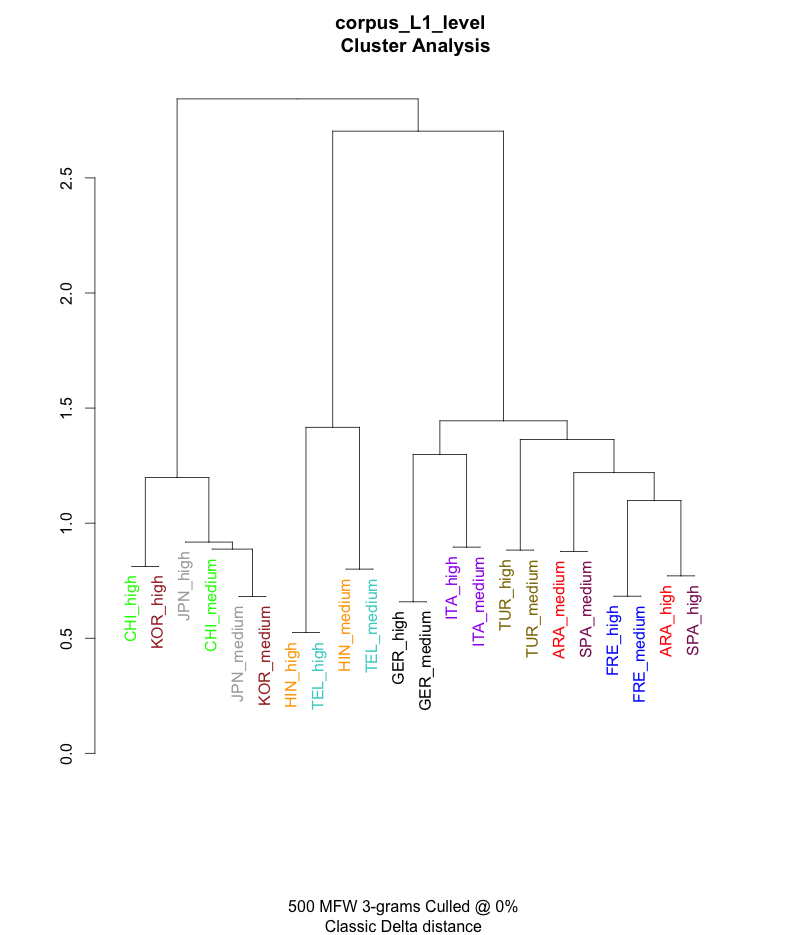
\includegraphics[width=0.8\textwidth,angle=-90]{clusteringexample.png}
\end{frame}

\begin{frame}
\frametitle{classification and clustering}
\begin{itemize}
\item Similarity: we have a collection of texts, we know what are the features we want to look for (words) \pause 
\item Difference: In the case of classification, we have a few examples classified into some categories, and we want the machine to learn to classify like this for new texts. \pause
\item In clustering, we do not have such examples, we have no idea how many groupings or possible. We want the machine to figure that out AND do the grouping. 
\end{itemize}
\end{frame}

\begin{frame}
\Large Topic Modeling
\end{frame}

\begin{frame}
\frametitle{Topic Modeling}
\begin{itemize}
\item Idea 1: each document is a mixture of topics
\item Idea 2: each topic can be represented by groups of words associated with it. \pause
\item Idea 3: a word may be very important in one topic, but may not be so important in another topic \pause
\item So how about looking at a collection of documents, extracting main topics from them and forming clusters of words based on topical similarity?
\end{itemize}
\end{frame}

\begin{frame}
\frametitle{Topic Modeling output - example}
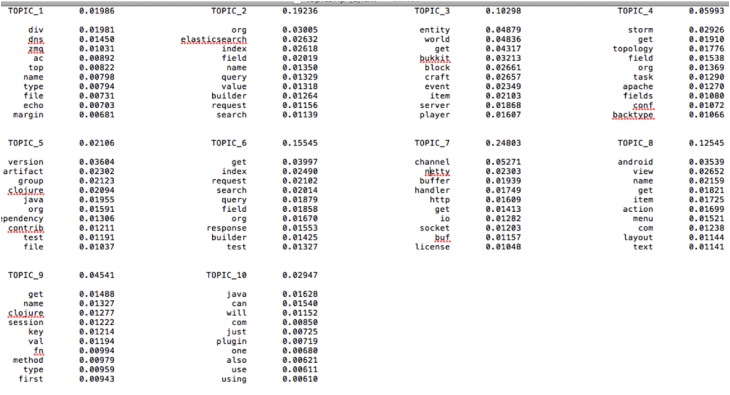
\includegraphics[width=0.9\textwidth]{topicmodeling.png}
\\ \tiny source: \url{http://shritir.weebly.com/uploads/2/6/3/4/26348989/2922455.png?1410730090}
\end{frame}

\begin{frame}
\frametitle{Topic Modeling output - another example}
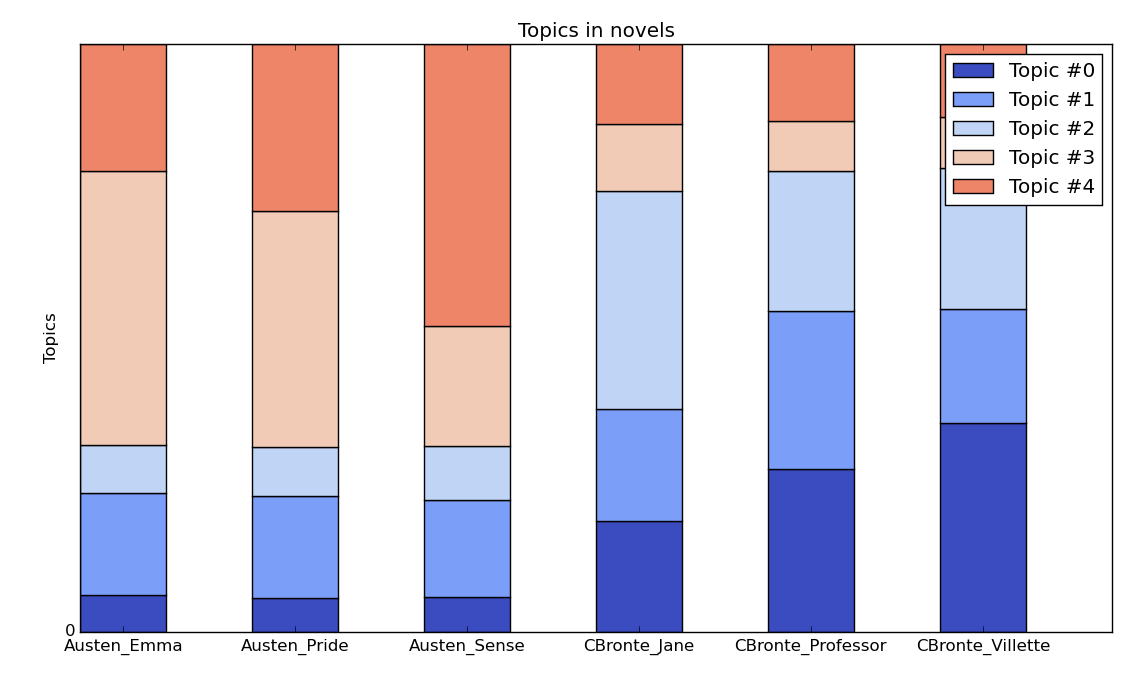
\includegraphics[width=0.9\textwidth]{topicmodeling2.png}
\\ \tiny source: \url{https://de.dariah.eu/tatom/_images/plot_doctopic_stacked_bar.png}
\end{frame}

\begin{frame}
\frametitle{clustering and topic modeling}
\begin{itemize}
\item Similarity: in both, we do not know what are the groups we are looking for and how many are they?  \pause 
\item Difference: In clustering, we generally talk about grouping texts together based on word patterns in them.\pause
\item In topic modeling, we generally talk about clustering words together based on the notion that all words in a cluster represent the vocabulary of a topic.
\end{itemize}
\end{frame}

\begin{frame}
\frametitle{Doing all these in R}
\begin{itemize}
\item There are several options.
\item tm is a popular library used to do such analysis, and there are several libraries that depend on this.
\item Textbook uses other libraries (different ones for different tasks)
\item I will use textbook examples where they are simpler, but make you work with tm for assignments (4--6). \pause
\item Assignments 4 and 5 are on text classification and topic modeling respectively, and you have to follow a R tutorial and write down reports.
\item Assignment 6 - you have to create some visualizations following instructions given. 
\end{itemize}
\end{frame}

\begin{frame}
\frametitle{How should we do all these in R?}
Typical steps: \small
\begin{itemize}
\item First, split your corpus into two groups: training data (to construct your model), testing data (to test your model accuracy)
\item Read in your collection of training texts (and their categories, if it is classification) \pause
\item Do your pre-processing (typical: lower casing, removing punctuations, removing numbers, removing "stop words", stemming) \pause
\item Create a term-document matrix \pause
\item Use this matrix along with any existing classification/clustering/topic modeling algorithm (100s of them exist. Some common algorithms for classification: naive bayes, support vector machines, decision trees, logistic regression etc.) \pause
\item Use this model to make predictions on the test data if it is classification
\item Figure out what to infer from topic clusters or document clusters otherwise
\end{itemize}
\end{frame}

\begin{frame}
\frametitle{Thursday}
\begin{itemize}
%\item Practical text classification: classifying movie reviews as positive or negative
%\item You can read some of the discussion in the textbook (chapter 12), but I will follow a simpler example.
\item Read these before coming to the class: 
\begin{enumerate}
\item \url{https://vvvvw.aaai.org/Papers/Workshops/1998/WS-98-05/WS98-05-001.pdf}
\item An encyclopaedia article I wrote recently, "Machine Learning and Applied Linguistics" just to get some perspective on real-world applications of this kind of macro analyses in a specific domain. It is uploaded on Canvas: Modules - Week 7
\end{enumerate}
\item Post a summary (3-4 bullet points) of each reading before you come on Thursday in the forum with Today's date.
\item We will continue this discussion, with some discussion exercises. 
\end{itemize}
\end{frame}

\end{document}

Thursday slides


